\begin{document}

\def\title{Worksheet 2}

\newcommand{\qitem}{\qpart\item}

\renewcommand{\labelenumi}{(\alph{enumi})} % change default enum format to (a)
\renewcommand{\theenumi}{(\alph{enumi})} % fix reference format accordingly.
\renewcommand{\labelenumii}{\roman{enumii}.} % second level labels.
\renewcommand{\theenumii}{\roman{enumii}.}

\maketitle

\vspace{0.5em}

\begin{qunlist}

% Author: Yannan Tuo, Varsha Ramakrishnan, Taejin Hwang
% Email: ytuo@berkeley.edu, vio@berkeley.edu, taejin@berkeley.edu
% Edited Lydia Lee, Spring 2019
% lydia.lee@berkeley.edu
% Edited: Justin Yu, Spring 2020
% justinvyu@berkeley.edu

\qns{Eigendecomposition and Change of Basis}

\meta{
  Please do a mini-lecture on change of basis similar to the opening paragraph of the change of coordinates question before doing this one.It is crucial that students understand change of basis, and how to convert from different bases first, before trying to understand eigendecomposition. It is up to you whether you want to mention the fact that all diagonalizable linear operators have a diagonal matrix representation given the correct choice of basis.
}

\textbf{Diagonal matrices}, matrices where all entries outside of the diagonal are zero, are often desirable since they are easy to analyze.
Determining properties such as rank and invertibility, are much simpler on a diagonal matrix as opposed to other non-diagonal matrices.
The process of \textbf{changing to a basis} in which the linear operator has a diagonal matrix representation is called \textbf{eigendecomposition} or \textbf{diagonalization.} You can think of eigendecomposition as a change of basis to one entirely made up of eigenvectors.

So what is a \textbf{change of basis}? Consider an arbitrary vector in $\mathbb{R}^2$: $\vec{x} = [ x_1 \text{ } x_2 ]^T$.
When we write a vector in this form, we are representing it as a linear combination of the \textit{standard basis} vectors for $\mathbb{R}^2$: $\vec{x} = x_1 \begin{bsmallmatrix} 1 \\ 0 \end{bsmallmatrix} + x_2 \begin{bsmallmatrix} 0 \\ 1 \end{bsmallmatrix}$. Naturally, $x_1$ and $x_2$ are the \textit{coordinates} of $\vec{x}$ in the standard basis (as you would refer to them if you graphed $\vec{x}$ on a Cartesian plane).

Now what if we wanted to represent that same vector in a different basis?
For example, say you wanted to represent the same vector $\vec{x}$ using the set of basis vectors $\vec{v_1}$ and $\vec{v_2}$.
This means that we need to find scalars $\alpha_1$ and $\alpha_2$ such that $\vec{x}$ can be written as a linear combination of these new basis vectors: $\vec{x} = \alpha_1 \vec{v_1} + \alpha_2 \vec{v_2}$.
To do this, we can just setup and solve a system of linear equations of the form:
$$\begin{bmatrix} \vec{v_1} & \vec{v_2} \end{bmatrix} \begin{bmatrix} \alpha_1 \\ \alpha_2 \end{bmatrix} = \begin{bmatrix} x_1 \\ x_2 \end{bmatrix}$$

In this problem, we'll investigate changing to and from the \textbf{eigenbasis} for the following matrix:

$$A = \begin{bmatrix}
2 & 2 \\
5 & -1
\end{bmatrix}$$

\begin{enumerate}

\qitem \textbf{Find $\lambda_1, \lambda_2$, the eigenvalues of $A$, ordered from largest to smallest.}
\ws{
\vspace{100px}
}

\meta {
  These first two parts are optional if students are comfortable with the process of finding eigenvalues and eigenspaces.
  It gives some concrete values that students can try out for the rest of the problem. If your students aren't convinced
  by $A = VDV^{-1}$, have them try out the concrete example with the numbers calculated in the first two parts.
}

\sol{
  \begin{align*}
    \text{det}(A - \lambda I) &= 0 \\
    (2 - \lambda) (-1 - \lambda) - 2(5) &= 0 \\
    \lambda^2 - \lambda - 12 &= 0 \\
    \implies \lambda_1 &= 4 \\
    \lambda_2 &= -3
  \end{align*}
}

\qitem \textbf{Find the eigenvectors $\vec{v_1}, \vec{v_2}$ corresponding to the eigenvalues.}

\ws{
\vspace{100px}
}

\sol{
  % \begin{bmatrix} 1 \\ 1 \end{bmatrix} \\ \begin{bmatrix} 1 \\ -1 \end{bmatrix}
  $$\vec{v_1} = \alpha \begin{bmatrix} 1 \\ 1 \end{bmatrix}$$
  $$\vec{v_2} = \beta \begin{bmatrix} -1 \\ -5/2 \end{bmatrix}$$
}

\end{enumerate}

With the eigenvectors we just found, define $V$ to be the matrix:
$$V = \begin{bmatrix}
\vec{v_1} & \vec{v_2}
\end{bmatrix}$$

\begin{enumerate}[resume]

\qitem Let $\widetilde{\vec{x}}$ be the coordinates of $\vec{x}$ in the eigenbasis. This means that for some arbitrary vector represented in the eigenbasis $\widetilde{\vec{x}} = \begin{bmatrix} \alpha_1 \\ \alpha_2 \end{bmatrix}$, the corresponding representation in standard coordinates is a linear combination of the columns of $V$: $\vec{x} = \alpha_1 \vec{v_1} + \alpha_2 \vec{v_2}$. \textbf{What is $\widetilde{\vec{x}}$ in terms of $V$ and $\vec{x}?$}

(\textit{Hint: Write $\vec{x}$ in terms of $V$ and $\tilde{\vec{x}}$, then go from there.})

\ws{\vspace{3em}}

\meta{
  The line $\alpha_1 \vec{v_1} + \alpha_2 \vec{v_2} = V \widetilde{\vec{x}}$ is not the most intuitive.
  It may require you showing on the board, why matrix vector multiplication can be seen as a linear combination of the columns.
}

\sol{
  $\vec{x} = \alpha_1 \vec{v_1} + \alpha_2 \vec{v_2} = V \widetilde{\vec{x}}.$ So it follows that $\widetilde{\vec{x}} = V^{-1} \vec{x}.$
}

\qitem It is often helpful to visualize the change of basis in a state diagram, where \textit{each arrow represents left-multiplying the variable it's coming out of by the corresponding matrix.} \textbf{Fill in the missing matrix operations in the state diagram based on your answer from the previous part.}

\ws {
  \begin{figure}[H]
    \centering
    \begin{tikzpicture}[node distance = 2cm, thick,every node/.style={inner sep=0.25em,outer sep=0.25em}]%
      \node (1) [circle,draw,minimum size=2em] {$\vec{x}$};
      \node (2) [circle,draw,right=of 1,minimum size=2em] {$\widetilde{\vec{x}}$};
      \draw[->] (1.45) -- node [rectangle,draw,midway,above,minimum size=2.5em] {} (2.135);
      \draw[->] (2.225) -- node [rectangle,draw,midway,below,minimum size=2.5em] {} (1.315);
    \end{tikzpicture}%
  \end{figure}
}

\meta {
  Not everyone finds this diagram the most intuitive, but it definitely helps a large percentage of students. Stress to students that it's always better to understand the intuitive meaning behind change of basis than to remember any particular change of basis formula. This intuitive meaning is bridging between coordinate systems, which can be visualized with this diagram.
}

\sol {
  \begin{figure}[H]
  \centering
  \begin{tikzpicture}[node distance = 2cm, thick,every node/.style={inner sep=0.25em,outer sep=0.25em}]%
    \node (1) [circle,draw,minimum size=2em] {$\vec{x}$};
    \node (2) [circle,draw,right=of 1,minimum size=2em] {$\widetilde{\vec{x}}$};
    \draw[->] (1.45) -- node [rectangle,draw,midway,above,minimum size=2.5em] {$V^{-1}$} (2.135);
    \draw[->] (2.225) -- node [rectangle,draw,midway,below,minimum size=2.5em] {$V$} (1.315);
  \end{tikzpicture}%
  \end{figure}
}


\qitem Now that we are able to switch back and forth between the coordinate systems, let's see how the linear transformation brought by $A$ can be viewed as a diagonal scaling transformation in the eigenbasis coordinate system.% Might be a bit confusing.

Let $\vec{y} = A \vec{x}$, and $\vec{x} = \alpha_1 \vec{v_1} + \alpha_2 \vec{v_2}$, using the same matrix $A$ and eigenvectors $\vec{v_1}, \vec{v_2}$ from before. Let $\widetilde{\vec{x}}$, $\widetilde{\vec{y}}$ be the coordinates of $\vec{x}$, $\vec{y}$ in the eigenbasis. \textbf{Find $\widetilde{\vec{x}}$ and $\widetilde{\vec{y}}$ in terms of $\alpha_1, \alpha_2, \lambda_1, \lambda_2$. What can we say about the relationship between $\widetilde{\vec{x}}$ and $\widetilde{\vec{y}}$?} % Might be confusing as to what the problem is asking compared to the next part.

(\textit{Hint}: Your answers shouldn't be in terms of the original $\vec{x}$ or $\vec{y}$.
 Use what you know about the coordinates of a vector in a certain basis; there is no need to invert any matrices or do any major computation.)

\ws {
  \vspace{100px}
}

\meta {
  Students may try to use what they found in the previous parts to multiply the vectors by $V^{-1}$. While this is technically right, make sure they understand what exactly
  that transformation is doing and why they don't need to do any matrix computation to find the coordinates of $\vec{y}$ in the eigenbasis.
}

\sol {
  $$\widetilde{\vec{x}} = \begin{bmatrix} \alpha_1 \\ \alpha_2 \end{bmatrix}$$

  \begin{align*}
    \vec{y} &= A \vec{x} \\
    &= A(\alpha_1 \vec{v_1} + \alpha_2 \vec{v_2}) \\
    &= \alpha_1 A \vec{v_1} + \alpha_2 A \vec{v_2} \\
    &= \alpha_1 \lambda_1 \vec{v_1} + \alpha_2 \lambda_2 \vec{v_2} \\
    \implies \widetilde{\vec{y}} &= \begin{bmatrix} \alpha_1 \lambda_1 \\ \alpha_2 \lambda_2 \end{bmatrix}
  \end{align*}

  This means that the matrix $D$ relating the two coordinates in the eigenbasis must be a diagonal scaling transformation, with the eigenvalues as the amount each dimension is scaled by.
}

\qitem \textbf{Find the matrix $D$ satisfying $\widetilde{\vec{y}} = D \widetilde{\vec{x}}$ in terms of $V$ and $A$.}

(\textit{Hint}: Start by writing $\vec{x}, \vec{y}$ in terms of $\widetilde{\vec{x}}$ and $\widetilde{\vec{y}}$. Refer to the state diagram from before.)

\ws{\vspace{120px}}

\meta {
  If students are comfortable with matrices representing linear transformations, you can explain this eigendecomposition as translating a linear transformation to and from the eigenbasis. For the diagonalization $A = VDV^{-1}$, left-multiplying an arbitrary vector $\vec{x}$ is equivalent to the following:

  \begin{align*}
    A \vec{x} &= VDV^{-1} \vec{x} \\
    &= VD \widetilde{\vec{x}} \\
    &= VD \begin{bmatrix} \alpha_1 \\ \alpha_2 \end{bmatrix} \\
    &= V \begin{bmatrix} \alpha_1 \lambda_1 \\ \alpha_2 \lambda_2 \end{bmatrix} \\
    &= V \widetilde{\vec{y}} \\
    &= \vec{y}
  \end{align*}
}

\sol {
  \begin{align*}
    \vec{y} &= A \vec{x} \\
    V \widetilde{\vec{y}} &= A V \widetilde{\vec{x}} \\
    \widetilde{\vec{y}} &= V^{-1} A V \widetilde{\vec{x}} \\
    \implies D &= V^{-1} A V
  \end{align*}
}

\qitem Finally, let's visualize this linear transformation $A$ from the perspective of two different coordinate systems in the state diagram below. \textbf{Fill in the missing matrix operations in the state diagram. How can you show and explain the diagonalization $A = VDV^{-1}$ (using the state diagram) and the change of basis perspective?}

\ws {
  \begin{figure}[H]
    \centering
    \begin{tikzpicture}[node distance = 2cm, thick, every node/.style={inner sep=0.25em,outer sep=0.25em}]%
      \node (1) [circle,draw,minimum size=2em] {$\vec{x}$};
      \node (2) [circle,draw,right=of 1,minimum size=2em] {$\vec{y}$};
      \node (3) [circle,draw,below=of 2,minimum size=2em] {$\widetilde{\vec{y}}$};
      \node (4) [circle,draw,below=of 1,minimum size=2em] {$\widetilde{\vec{x}}$};
      \draw[->] (1) -- node [rectangle,draw,midway,above,minimum size=2.5em] {} (2);
      \draw[->] (1.240) -- node [rectangle,draw,midway,left,minimum size=2.5em]{} (4.120);
      \draw[->] (4.60) -- node [rectangle,draw,midway,right,minimum size=2.5em]{} (1.300);
      \draw[->] (2.300) -- node [rectangle,draw,midway,right,minimum size=2.5em]{} (3.60);
      \draw[->] (3.120) -- node [rectangle,draw,midway,left,minimum size=2.5em]{} (2.240);
      \draw[->] (4) -- node [rectangle,draw,midway,below,minimum size=2.5em] {} (3);
    \end{tikzpicture}%
  \end{figure}
}

\sol {
  \begin{figure}[H]
    \centering
    \begin{tikzpicture}[node distance = 2cm, thick, every node/.style={inner sep=0.25em,outer sep=0.25em}]%
      \node (1) [circle,draw,minimum size=2em] {$\vec{x}$};
      \node (2) [circle,draw,right=of 1,minimum size=2em] {$\vec{y}$};
      \node (3) [circle,draw,below=of 2,minimum size=2em] {$\widetilde{\vec{y}}$};
      \node (4) [circle,draw,below=of 1,minimum size=2em] {$\widetilde{\vec{x}}$};
      \draw[->] (1) -- node [rectangle,draw,midway,above,minimum size=2.5em] {$A$} (2);
      \draw[->] (1.240) -- node [rectangle,draw,midway,left,minimum size=2.5em]{$V^{-1}$} (4.120);
      \draw[->] (4.60) -- node [rectangle,draw,midway,right,minimum size=2.5em]{$V$} (1.300);
      \draw[->] (2.300) -- node [rectangle,draw,midway,right,minimum size=2.5em]{$V^{-1}$} (3.60);
      \draw[->] (3.120) -- node [rectangle,draw,midway,left,minimum size=2.5em]{$V$} (2.240);
      \draw[->] (4) -- node [rectangle,draw,midway,below,minimum size=2.5em] {$D$} (3);
    \end{tikzpicture}%
  \end{figure}

  You can explain $A = VDV^{-1}$ by just left-multiplying in the order of the arrows from $\vec{x}$ to $\vec{y}$. Again, in the change of basis perspective, $V^{-1}$ first pulls the vector $\vec{x}$ into the eigenbasis. $D$ performs the equivalent linear transformation of $A$ but in the eigen-coordinate system. Finally, $V$ brings the transformed vector back into standard coordinates.
}

% \qitem In the standard basis, we currently have the input output relation: $\vec{y} = D \vec{x}.$
% Using a change of coordinates, how can we represent our original diagonal matrix as an input-output relationship in the basis S?
% That is, if $[\vec{y}]_S = A [\vec{x}]_S,$ how would you represent $A?$

% \sol {
%   We start with the current conversion between standard and S-coordinates.
%   \begin{gather*}
%     \vec{x} = V [\vec{x}]_S, \vec{y} = V [\vec{y}]_S
%   \end{gather*}

%   Then substituting in for the original relation $\vec{y} = D \vec{x},$ we get:
%   $$V[\vec{y}]_S = D V[\vec{x}]_S$$

%   Left multiplying by $V^{-1}$ we see that:
%   $$[\vec{y}]_S = V^{-1} D V[\vec{x}]_S$$

%   So it follows that $A = V^{-1} D V$
% }

% \qitem Now we will look at the case in which we start with the matrix
% $$ A = \begin{bmatrix}
%         1 & 4 \\
%         2 & 3
%   \end{bmatrix} $$
% represented in the standard basis. What are the eigenvalues of $A?$ Order from largest to smallest.

% \sol {
%   In order to find the eigenvalues of $A,$ we look at the determinant of $A - \lambda I.$
%   $$det\mathbf{\begin{bmatrix}
%   1-\lambda & 4 \\
%   2 & 3-\lambda
%  \end{bmatrix}}  =  (1 - \lambda)(3 - \lambda) - 8 =  \lambda^2 - 4 \lambda - 5 = 0$$
%  $$ \lambda_1 = 5, \lambda_2 = -1$$
% }

% \qitem What is a basis for the eigenspace for $\lambda_1$ and $\lambda_2?$

% \sol {
%   To find the eigenspaces for $\lambda$ we compute the null-spaces of $A - \lambda I.$
%   $$A - 5I = \begin{bmatrix}
%   -4 & 4 \\
%   2 & -2
%  \end{bmatrix}$$
%  We can see that $\begin{bmatrix} 1 \\ 1 \end{bmatrix}$ is a basis for the null-space of $A - 5I.$

%  $$A + I = \begin{bmatrix}
%   2 & 4 \\
%   2 & 4
%  \end{bmatrix}$$
%  We can see that $\begin{bmatrix} -2 \\ 1 \end{bmatrix}$ is a basis for the null-space of $A + I.$
% }

% \qitem What do you notice about the eigenvalues and eigenvectors of $A?$

% \sol {
%   The eigenvectors of $A$ are the same vectors as the vectors in the basis $S.$ \\
%   The eigenvalues of $A$ have the same values as the diagonal entries of the matrix $D.$ \\
%   This should not be a coincidence. This is because $A$ is in fact a linear operator with a diagonal matrix representation "hidden" under the eigenbasis.
% }

% \qitem In the standard basis, we currently have the input output relation: $\vec{y} = A \vec{x}.$
% Using a change of coordinates, how can we represent our original diagonal matrix as an input-output relationship in the basis S?
% That is, if $[\vec{y}]_S = B [\vec{x}]_S,$ how would you represent $B?$ Try to do the calculation as well.

% \meta{
%   If you don't do end up doing the calculation, at least write out the matrices A and V as you're doing this, and state that $B = D$ at the end.
% }

% \sol {
%   We start with the current conversion between standard and S-coordinates.
%   \begin{gather*}
%     \vec{x} = V [\vec{x}]_S, \vec{y} = V [\vec{y}]_S
%   \end{gather*}

%   Then substituting in for the original relation $\vec{y} = A \vec{x},$ we get:
%   $$V[\vec{y}]_S = A V[\vec{x}]_S$$

%   Left multiplying by $V{-1}$ we see that:
%   $$[\vec{y}]_S = V^{-1} A V[\vec{x}]_S$$

%   So it follows that $B = V^{-1} A V.$ \vskip 1pt
%   However after doing the calculation, we see that $B = D!$
% }

% \qitem What is the relationship between $A, D$ and $V?$ In other words, how can you express $A$ using $D$ and $V?$

% \sol {
%   We saw from the previous part that $D = V^{-1} A V.$
%   Therefore, $A = V D V^{-1}.$
% }

% \qitem When can a matrix not be diagonalized?
% In other words, when does a linear operator not have a diagonal matrix representation?

% \sol {
%   A linear operator cannot have a diagonal matrix representation if it isn't possible to change to a basis made up of eigenvectors.
%   Remember that a change of coordinates matrix must be invertible.
%   However, if a matrix does not have $n$ linearly independent eigenvectors, then it cannot have a change of basis matrix.
% }

\end{enumerate}

\newpage
% {\Large \textbf{Mechanical:}}
\qns{An Introduction to Systems}

\meta{You may want to write out the differential equation as:
$$\ddt{}{t} \vec{x}(t) = \ddt{}{t} \begin{bmatrix} x_1 \\ \vdots \\ x_n \end{bmatrix} = \begin{bmatrix} f_1(x_1, .., x_n) \\ \vdots \\ f_n(x_1, .., x_n) \end{bmatrix}$$
}

In the next couple of problem sets, we will be examining systems. 
Many physical systems such as the motion of a car, can be modeled using a system.
Often times, when we are describing a system, we will have a \textbf{state variable $\vec{x},$}
that will often be a multivariable function. 

For a given system, we can often write a differential equation describing its change over time as
\begin{align}
\ddt{\vec{x}(t)}{t} = A \vec{x}(t) + \vec{b}
\end{align}

This differential equation is referred to as a \textbf{vector differential equation} 
and is a generalization of single variable differential equations to the multivariate case.
In this context, $A$ is a $n \times n$ matrix, and $\vec{b}$ is a scalar vector in $\mathbb{R}^n.$

Given the following system:
\begin{align*}
    \ddt{}{t}x_{1}(t) &= 3 x_{1}(t) - 2 x_{2}(t) \\
    \ddt{}{t}x_{2}(t) &= - x_{1}(t) + 5 x_{2}(t)
\end{align*}

With initial conditions $x_{1}(0) = 2, \ x_{2}(0) = 3,$

\begin{enumerate}
    \qitem What is an appropriate state vector for this system?

    \sol{
        We have to variables $x_1$ and $x_2$ therefore we define our state vector as:
        $$\vec{x} = \begin{bmatrix} x_{1} \\ x_{2} \end{bmatrix}$$
    }

    \qitem What is the initial condition of this system?

    \sol{
        We have the individual initial conditions for $x_1$ and $x_2$ but we must also a define an initial condition for our state vector.
        $$\vec{x}(0) = \begin{bmatrix} x_{1}(0) \\ x_{2}(0) \end{bmatrix} = \begin{bmatrix} 2 \\ 3 \end{bmatrix} $$
    }

    \qitem Write out the system of differential equations as a vector differential equation.
    
    \sol{
        $$\ddt{}{t}\vec{x}(t) = \begin{bmatrix} 3 & -2 \\ -1 & 5 \end{bmatrix} \begin{bmatrix} x_{1}(t) \\ x_{2}(t) \end{bmatrix} 
        = \begin{bmatrix} 3 & -2 \\ -1 & 5 \end{bmatrix} \vec{x}(t) $$
    }
\end{enumerate}

% \qitem Explain why the system 
%     \begin{align*}
%         \ddt{x}{t} &= ax + by \\
%         \ddt{y}{t} &= cx + dy
%     \end{align*}
%     can be equivalently formulated as
%     \[
%         \ddt{}{t} \begin{bmatrix} x \\ y \end{bmatrix} = \begin{bmatrix} a & b \\ c & d \end{bmatrix} \begin{bmatrix} x \\ y \end{bmatrix}
%     \]


% \qitem Given the following system:
%     \begin{align*}
%         \ddt{x}{t} &= x \\
%         \ddt{y}{t} &= y
%     \end{align*}

%     With initial conditions $x(0) = x_0, \ y(0) = y_0,$

%     \begin{enumerate}
%         \qitem What is an appropriate state vector for this system?
%         \qitem What is the initial condition of this system?
%         \qitem Convert this system into its State-space representation.
%         \qitem How can you solve for $x(t)$ and $y(t)?$
%     \end{enumerate}

\newpage
\qns{Multivariate ODE with Coordinate Changes}
\qcontributor{Anant Sahai}
\qcontributor{Regina Eckert}
\qcontributor{Elena Jia}

\begin{enumerate}

\qitem Consider a system of differential equations (valid for
$t\geq 0$)
\begin{equation}
\frac{d}{dt}y_1(t) = 5 y_1(t) + 2 y_2(t)
\end{equation}
\begin{equation}
\frac{d}{dt}y_2(t) = -8 y_1(t) -5 y_2(t)
\end{equation}

with initial conditions $y_1(0) = 3$ and $y_2(0) = 3$.

Write out the differential equations and initial conditions in matrix/vector form.

\meta{
TA Guidance: Explain that usually they will be getting problems in this form. 

The general procedure for solving this type of problem is: \\
First, convert to the eigenbasis. Solve the problem there. Then convert back to the problem basis to find the final answer.
}

\sol{
	$$\begin{bmatrix}\frac{d}{dt}y_1(t) \\ \frac{d}{dt}y_2(t)\end{bmatrix} = \begin{bmatrix}5 & 2 \\ -8 & -5\end{bmatrix}\begin{bmatrix}y_1(t) \\ y_2(t)\end{bmatrix}$$
	
$$\begin{bmatrix}y_1(0) \\ y_2(0)\end{bmatrix} =\begin{bmatrix}3 \\ 3\end{bmatrix} $$

We will define the differential matrix as $A_y$, where 

$$A_y = \begin{bmatrix}5 & 2 \\ -8 & -5\end{bmatrix} $$
} 

\bigskip

\begin{adjustwidth}{-20pt}{0pt}
	We already know how to solve the system of differential equations if $\frac{d}{dt}y_1(t)$ only depends on $y_1(t)$ and $\frac{d}{dt}y_2(t)$ only depends on $y_2(t)$.
	However, we can't directly solve a system of ODEs where $\frac{d}{dt}y_1(t)$ and $\frac{d}{dt}y_2(t)$ each depend on both $y_1(t)$ and $y_2(t)$. \\
	The solution? Change coordinates to the eigenbasis to diagonalize our transformation matrix.\\
	Then, we will have $\frac{d}{dt}z_{\lambda_1}(t) = \lambda_1 z_{\lambda_1}(t)$ and $\frac{d}{dt}z_{\lambda_2}(t) = \lambda_2 z_{\lambda_2}(t)$, which we know how to solve.
	
\end{adjustwidth}



\qitem Find the eigenvalues $\lambda_1, ~\lambda_2$ and eigenspaces for the differential equation matrix above.

\meta{
TA Guidance:  The determinant is something that finds the
oriented volume of the matrix acting on the standard unit cube
(represented by the identity matrix). This is what they have been
taught about determinants in 16A. As a result, if a matrix has a
nontrivial nullspace, there are directions that it maps to zero. 
\medskip
As a result, it ``squashes'' things that have volume into pancakes or
lines or dots that have no volume. Consequently, the determinant of
a matrix with a nontrivial nullspace must be zero. 
\medskip
Fortunately, the
determinant of a matrix can be easily computed via Gaussian
Elimination (since every step in Gaussian elimination has an
interpretation in terms of what it does to oriented volume --- a
swap of rows negates the sign of the oriented volume (since this is
like looking into a mirror.); scaling a row
scales the oriented volume by the same amount, and adding a multiple
of one row to another does nothing to oriented volumes (for the
same reason that pushing a deck of cards does nothing to its
volume).
\medskip 

They also know that this Gaussian elimination approach can be
done directly on simple symbolic 2x2 and 3x3 matrices to give the
simple formulas that we know. They barely know that the determinant is
the product of its eigenvalues, although that clearly makes sense from
this perspective. That's about all they know about determinants from
16A. 
\medskip
They do not know the cofactor formulas nor do they know the
signed permutation interpretation nor the alternating linear forms
interpretation. Those topics are viewed as voodoo at the maturity
level of 16 students (they would just memorize them without
understanding, so why teach something that they cannot truly
understand) and so are not to be invoked.

}

\sol{
	Eigenvalues $\lambda$ and eigenvectors $v$ of matrix $A$ are given by
	
	$$A_yv = \lambda v$$
	In order to find the eigenvalues, we take the determinant:
	
$$\text{det}\left( A-\lambda I \right) = 0$$

$$\text{det}\left( \begin{bmatrix}5-\lambda & 2 \\ -8 & -5-\lambda\end{bmatrix} \right) = 0$$

We can solve this using a $2 \times 2$ determinant form seen in 16A,

$$\text{det}\left( \begin{bmatrix}a & b \\ c & d\end{bmatrix} \right) = ad - bc,$$

or by Gaussian elimination. \\
This produces the characteristic polynomial of the matrix:

\begin{align*}
(-5-\lambda)(5-\lambda) + 16 &=0 \\
% 12 + 7\lambda + \lambda^2 -2 &=0 \\
% \lambda ^2 + 7\lambda + 10 & = 0 \\
(\lambda + 3)(\lambda -3) &= 0	
\end{align*}

Giving:

$$\lambda = 3, -3$$

The eigenspace associated with $\lambda_1 = -3$ is given by the span of the eigenvector $\vec v_{\lambda_1}$:

	 $$ \begin{bmatrix}-4 + 5 & 1 \\ 2 & -3 + 5\end{bmatrix} \vec v_{\lambda_1} = \begin{bmatrix}0 \\ 0\end{bmatrix}$$
	 	$$ \begin{bmatrix}1 & 1 \\ 2 & 2\end{bmatrix} \vec v_{\lambda_1} = \begin{bmatrix}0 \\ 0\end{bmatrix}$$
	 $$\vec v_{\lambda_1}=
	 \begin{bmatrix} -1 \\ 4\end{bmatrix} $$

The eigenspace associated with $\lambda_2 = 3$ is given by the span of the eigenvector $\vec v_{\lambda_2}$:
	
	 $$ \begin{bmatrix} 
	 -4 + 2 & 1 \\ 
	 2 & -3 + 2
	 \end{bmatrix} 
	 \vec v_{\lambda_2} = 
	 \begin{bmatrix}0 \\ 0\end{bmatrix}
	 $$
	 $$ \begin{bmatrix}
	 	-2 & 1 \\ 
		2 & -1
	\end{bmatrix} 
	\vec v_{\lambda_2} = \begin{bmatrix} 0 \\ 0\end{bmatrix}$$
	$$\vec v_{\lambda_2}=
	\begin{bmatrix} -1 \\ 1\end{bmatrix} $$

}


\qitem Change coordinates into the eigenbasis to re-express the
differential equations in terms of new variables $z_{\lambda_1}(t), ~
z_{\lambda_2}(t)$. (These variables represent eigenbasis-aligned coordinates.) \\
\textit{
 i.e. find a matrix A' such that $\frac{d}{dt} \vec{z_{\lambda}} = A' \vec{z_{\lambda}}$
} \\

\sol{
		\begin{centering}
	\begin{tikzpicture}
	
	\draw (-1,0) node[anchor = east] {$z_{\lambda_i}$ coordinates};
	\draw (0,0) circle (0.5cm);
	\draw (-1,2) node[anchor = east] {$y_i$ coordinates};
	\draw[->] (0,0.5) -- (0,1.5) node[anchor=north east] {$V$};
	\draw (0,2) circle (0.5cm);
	\draw[->] (0.5,2) -- (4.5,2) node[anchor=south east] {$ A_y = \begin{bmatrix}5 & 2 \\ -8 & -5\end{bmatrix}$} ;
	\draw (3,2) node[anchor=north] {differentiation};
	\draw (5,2) circle (0.5cm);
	\draw[->] (5,1.5) -- (5,0.5) node[anchor=south west] {$V^{-1}$};
	\draw (5,0) circle (0.5cm);
	\draw[dashed,->] (0.5,0) -- (4.5,0) node[anchor=south east] {$ A_{z_\lambda} =V^{-1} A V$} ;
	
	\end{tikzpicture}
\end{centering}

$$\vec y =\vec v_{\lambda_1} z_{\lambda_1} + \vec v_{\lambda_2} z_{\lambda_2}$$
$$\vec y =\begin{bmatrix} -1 & -1 \\ 4 & 1\end{bmatrix}\begin{bmatrix}z_{\lambda_1} \\ z_{\lambda_2}\end{bmatrix}$$

We can define the change-of-coordinates matrix from the eigenbasis to our original basis as 

$$V=\begin{bmatrix} -1 & -1 \\ 4 & 1\end{bmatrix}$$

Changing coordinates to the eigenbasis:

$$\begin{bmatrix}z_{\lambda_1} \\ z_{\lambda_2}\end{bmatrix} = V^{-1}\begin{bmatrix}y_1 \\ y_2\end{bmatrix}   $$

$$V^{-1}=\begin{bmatrix}\frac{1}{3} & \frac{1}{3} \\ -\frac{4}{3} & -\frac{1}{3}\end{bmatrix}$$

$$A_{z_\lambda} = V^{-1} A_y V = \begin{bmatrix}\frac{1}{3} & \frac{1}{3} \\ -\frac{4}{3} & -\frac{1}{3}\end{bmatrix}\begin{bmatrix}5 & 2 \\ -8 & -5\end{bmatrix}\begin{bmatrix} -1 & -1 \\ 4 & 1\end{bmatrix}$$
% $$A_{z_\lambda} = \begin{bmatrix}\frac{2}{3} & -\frac{1}{3} \\ \frac{1}{3} & \frac{1}{3}\end{bmatrix}\begin{bmatrix}-5 & -2 \\ 5 & -4\end{bmatrix}$$
$$A_{z_\lambda} = \begin{bmatrix}-3 & 0 \\ 0 & 3\end{bmatrix}$$

That is:

	$$\begin{bmatrix}\frac{d}{dt}z_{\lambda_1}(t) \\ \frac{d}{dt}z_{\lambda_2}(t)\end{bmatrix} = \begin{bmatrix}-3 & 0 \\ 0 & 3\end{bmatrix}\begin{bmatrix}z_{\lambda_1}(t) \\ z_{\lambda_2}(t)\end{bmatrix}$$


}

\qitem Solve the differential equation for $z_{\lambda_i}(t)$ in the eigenbasis.

\sol{
First we get the initial condition:

$$\vec z_{\lambda}(0) = \begin{bmatrix}\frac{1}{3} & \frac{1}{3} \\ -\frac{4}{3} & -\frac{1}{3}\end{bmatrix}\begin{bmatrix} 3 \\ 3 \end{bmatrix} = \begin{bmatrix} 2 \\ -5 \end{bmatrix} $$

Then we solve based on the form of the problem and our previous differential equation experience:

$$\vec z_{\lambda}(t) = \begin{bmatrix} K_1 e^{-3t} \\ K_2 e^{3t} \end{bmatrix} $$

Plugging in for the initial condition gives:

$$\vec z_{\lambda}(t) = \begin{bmatrix} 2 e^{-3t} \\ -5 e^{3t} \end{bmatrix} $$

}

\qitem Convert your solution back into the original coordinates to find $y_i(t)$.

\sol{
$$ \vec y(t) = V \vec z_{\lambda}(t) =  \begin{bmatrix} -1 & -1 \\ 4 & 1\end{bmatrix}\begin{bmatrix} 2 e^{-3t} \\ -5 e^{3t}  \end{bmatrix} = \begin{bmatrix} -2e^{-3t} + 5 e^{3t}\\ 8e^{-3t}-5e^{3t} \end{bmatrix}$$
}


\qitem We can solve this equation using a slightly shorter approach by observing that the solutions for $y_i(t)$ will all be of the form
$$y_i(t) = \sum_k K_{i,k} e^{\lambda_k t}$$

where $\lambda_k$ is an eigenvalue of our differential equation
relation matrix and the $K_{i,k}$ are constants derived from our
initial conditions and the coordinate changes involved. 

Since we have observed that the solutions will include
$e^{\lambda_i t}$ terms, once we have found the eigenvalues for our
differential equation matrix, we can guess the forms of the $y_i(t)$ as

 	$$\begin{bmatrix}y_1(t) \\ y_2(t)\end{bmatrix}
        = \begin{bmatrix}\alpha e^{\lambda_1t} + \beta e^{\lambda_2t}
          \\ \gamma e^{\lambda_1 t}  + \kappa e^{\lambda_2 t} \end{bmatrix}$$
where $\alpha, ~\beta, ~\gamma, ~\kappa$ are all constants.

\begin{enumerate}
	\qitem Take the derivative to write out 
	$$\begin{bmatrix}\frac{d}{dt}y_1(t) \\ \frac{d}{dt}y_2(t)\end{bmatrix}.$$ in matrix-vector form.
	
	\sol{
	 	$$\begin{bmatrix}y_1(t) \\ y_2(t)\end{bmatrix} = \begin{bmatrix}\alpha e^{-3t} + \beta e^{3t}  \\ \gamma e^{-3t}  + \kappa e^{3t} \end{bmatrix}$$
		$$\frac{d}{dt} \vec y(t) = \begin{bmatrix}-3\alpha e^{-3t} +3 \beta e^{3t}  \\ -3\gamma e^{-3t} + 3 \kappa e^{3t} \end{bmatrix}$$
		If we notice that the right-hand side can be written as linear combinations of $e^{-3t}$ and $e^{3t}$, we can write the previous equation as:
		$$ \frac{d}{dt} \vec y(t) = 
		\begin{bmatrix}
			-3 \alpha & 3 \beta  \\ -3 \gamma & 3 \kappa
		\end{bmatrix}
		\begin{bmatrix}
			e^{-3t} \\ e^{3t}
		\end{bmatrix}
		$$
	}
	
	\qitem Connect this differential equation to the matrix-vector equation you found in part (a).\\
	\sol{
		$$\frac{d}{dt} \vec y(t) = 
		\begin{bmatrix}
			5 & 2 \\ 
			-8 & -5
		\end{bmatrix}
		\vec{y}(t) = 
		\begin{bmatrix}
			-3 \alpha & 3 \beta  \\ -3 \gamma & 3 \kappa
		\end{bmatrix}
		\begin{bmatrix}
			e^{-3t} \\ e^{3t}
		\end{bmatrix} 
		$$
		Substituting
		$$ \begin{bmatrix}
			\alpha e^{-3t} + \beta e^{3t}  \\ \gamma e^{-3t}  + \kappa e^{3t} 
		\end{bmatrix} = 
		\begin{bmatrix}
			\alpha & \beta  \\ \gamma & \kappa
		\end{bmatrix}
		\begin{bmatrix}
			e^{-3t} \\ e^{3t}
		\end{bmatrix}
		$$
		for $\vec{y}(t)$, we get:
		$$
		\begin{bmatrix}
			5 & 2 \\ 
			-8 & -5
		\end{bmatrix} 
		\begin{bmatrix}
			\alpha & \beta  \\ \gamma & \kappa
		\end{bmatrix}
		\begin{bmatrix}
			e^{-3t} \\ e^{3t}
		\end{bmatrix} = 
		\begin{bmatrix}
			-3 \alpha & 3 \beta  \\ -3 \gamma & 3 \kappa
		\end{bmatrix}
		\begin{bmatrix}
			e^{-3t} \\ e^{3t}
		\end{bmatrix} 
		$$		
		Doing the matrix multiplication on the left-hand side of the equation, we get:
		$$
		\begin{bmatrix}
			5 \alpha + 2 \gamma & 5 \beta + 2 \kappa \\ 
			-8 \alpha - 5 \gamma & -8 \beta - 5 \kappa
		\end{bmatrix} 
		\begin{bmatrix}
			e^{-3t} \\ e^{3t}
		\end{bmatrix} = 
		\begin{bmatrix}
			-3 \alpha & 3 \beta  \\ -3 \gamma & 3 \kappa
		\end{bmatrix}
		\begin{bmatrix}
			e^{-3t} \\ e^{3t}
		\end{bmatrix} 
		$$		
	}
	
	\qitem Use what you found in the previous step to solve for $\gamma$ and $\kappa$ in terms of $\alpha$ and $\beta$, respectively. \\
	\sol {
		Equating terms in the matrices on the left- and right-hand sides of the equation, we get:
		$5 \alpha + 2 \gamma = -3 \alpha$, 
		$5 \beta + 2 \kappa = 3 \beta$,
		$-8 \alpha - 5 \gamma = -3 \gamma$, and 
		$-8 \beta - 5 \kappa = 3 \kappa$.
		
		From the first equation, we get $\gamma = -4 \alpha$. From the second, we get $\kappa = - \beta$. \\
		We could get the same result from using the third and fourth equations. 
	}
	
	\qitem Use initial conditions to finish solving for $\vec{y}(t)$. \\
	\sol {
		From the initial condition, we have:
		$$\vec{y}(0) = 
		\begin{bmatrix} 3 \\ 3 \end{bmatrix} = 
		\begin{bmatrix}
			\alpha & \beta  \\ \gamma & \kappa
		\end{bmatrix}
		\begin{bmatrix}
			e^{-3 \cdot 0} \\ e^{3 \cdot 0}
		\end{bmatrix} = 
		\begin{bmatrix}
			\alpha & \beta  \\ \-4 \alpha & - \beta
		\end{bmatrix}
		\begin{bmatrix}
			1 \\ 1
		\end{bmatrix}$$
		From this, we get the equations $\alpha + \beta = 3$ and $-4 \alpha - \beta = 3$.
		$$\alpha=-2$$
	 	$$\beta=5$$
		
		We can now plug in our 4 constants to find $\vec{y}(t)$:
		$$\begin{bmatrix}y_1(t) \\ y_2(t)\end{bmatrix} = \begin{bmatrix} -2e^{-3t} + 5e^{3t}  \\ 8e^{-3t}  -5  e^{3t} \end{bmatrix}$$
		Note that this is the same as the answer from part (e)
	}
\end{enumerate}

\end{enumerate}	
\newpage
\qns{RLC circuit}

Consider the circuit shown below:

\begin{center}
    \begin{circuitikz}[scale=0.8]
        \draw (-1,4)
        to [V = $V_s$,i=$i_s$] (-1,0)
        (-1,4) to [switch, l^=\mbox{$t = 0$} ] (1,4)
        to [opening switch,l^=\mbox{$t = 0$} ] (1,0)
        (1,4) to [R = $R_s$] (4,4)
        to [C = $C$,i=$i_C$] (4,0)
        to [short] (-1,0)
        (4,4) to [short] (8,4)
        to [L = $L$,i=$i_L$, v = $V_{out}$] (8,0)
        to [short] (-1,0);
    \end{circuitikz}
\end{center}

Assume the circuit reaches steady state for $t<0.$ At time $t = 0,$ the switch changes state and connects to the \text{bf}{constant} voltage source $V_s$.

\meta {
    Explain what it means when the circuit reaches steady state.
}

\begin{enumerate}

	\qitem \textbf{Find the differential equation for $V_{out}$ for $t\geq0$.} \textit{Hint: Write out the KCL equation.}

    \ws {
        \vspace{120px}
    }

	\meta {
		It might not be intuitive at first to take the derivative, however, we want to find $V_{out} = V_L$ and remember that the voltage-current relationship of an inductor is $V_L = L \ddt{i_L(t)}{t}.$
		Our KCL equation is in terms of $i_L(t)$ we'll take a derivative to substitute the relation above.
	}

	\sol{
	We first see that
	$$i_s = i_R = i_C + i_L$$
	We will take the derivative to get:
	$$\ddt{i_s}{t} = \ddt{i_C}{t} + \ddt{i_L}{t}$$
	From the voltage-current relations, we know that:
	$$i_s = \frac{V_s-V_{out}}{R_s}, i_C = C \ddt{V_{out}}{t}, \ddt{i_L(t)}{t} = \frac{V_{out}}{L}$$
	Taking derivatives and substituting we get:
	$$\frac{d^2V_{out}}{dt^2}+\frac{1}{R_sC}\frac{dV_{out}}{dt}+\frac{1}{LC}V_{out} = 0$$
% \[i_s=i_c+i_l\]
% Using $i_c=C\frac{dV_{out}}{dt}$ and Ohm's law:
% \[\frac{V_s-V_{out}}{R_s}=C\frac{dV_{out}}{dt}+i_l\]

% Substituting $V_{out}=L\frac{di_l}{dt}$
% \[\frac{V_s}{R_s}=\frac{L}{R_s}\frac{di}{dt}+LC\frac{d^2i}{dt^2}+i_l\]
% \[\frac{V_s}{R_sLC}=\frac{1}{R_sC}\frac{di}{dt}+\frac{d^2i}{dt^2}+\frac{i_l}{LC}\]
% Since we have $V_{out}=L\frac{di_l}{dt}$, we take the derivative of both sides to get an equation in the form of $V_{out}$
% \[0=\frac{1}{R_sC}\frac{d^2i}{dt^2}+\frac{d^3i}{dt^3}+\frac{1}{LC}\frac{di_l}{dt}\]
% \[0=\frac{d^2V_{out}}{dt^2}+\frac{1}{R_sC}\frac{dV_{out}}{dt}+\frac{1}{LC}V_{out}\]
    }
    \qitem We will define our state variable $\vec{x}(t) = \begin{bmatrix} V_{out}(t) \\ \frac{d}{dt} V_{out}(t) \end{bmatrix}$.

    \textbf{Set up a system of differential equations in the form $\frac{d}{dt}\vec{x}(t) = A \vec{x}(t)$. What are its initial conditions $\vec{x}(0)$?}

    \ws{
        \vspace{120px}
    }
    \sol{
    We know that at $t=0,$ $V_{out}=0$, $i_C=0$, and $i_L=0$. We also know that the voltage on a capacitor and the current through an inductor can't change instantaneously, so it follows that
    $$\vec{x}(0) = \begin{bmatrix} V_{out}(0)=0 \\ \ddt{V_{out}(t)}{t}(0)=0 \end{bmatrix}.$$
    Putting the differential equation in state-space we see that:
    $$\ddt{}{t} \vec{x}(t) =
    \begin{bmatrix} \ddt{V_{out}(t)}{t} \\ \frac{d^2V_{out}}{dt^2} \end{bmatrix} =
    \begin{bmatrix} \ddt{V_{out}(t)}{t} \\ -\frac{1}{R_sC} \frac{dV_{out}}{dt} - \frac{1}{LC} V_{out} \end{bmatrix} =
    \begin{bmatrix} 0 & 1 \\ -\frac{1}{LC} & -\frac{1}{R_sC} \end{bmatrix}\begin{bmatrix} V_{out}(t) \\ \ddt{V_{out}(t)}{t} \end{bmatrix} =\begin{bmatrix} 0 & 1 \\ -\frac{1}{LC} & -\frac{1}{R_sC} \end{bmatrix} \vec{x}$$
    }

	\qitem \textbf{Find the eigenvalues of $A$.}

    \ws {
        \vspace{120px}
    }

    \sol {
    To find the eigenvalues, we take a look at the determinant of $A - \lambda I.$
    $$\text{det}\mathbf
    {\begin{bmatrix}
        -\lambda & 1 \\
        -\frac{1}{LC} & -\frac{1}{R_s C} - \lambda \end{bmatrix}}
    = (- \lambda)(-\frac{1}{R_s C} - \lambda) + \frac{1}{LC} = \lambda^2 + \frac{1}{R_s C} \lambda + \frac{1}{LC}$$
    Therefore using the quadratic formula,
    $$\lambda = -\frac{1}{2 R_s C} \pm \frac{1}{2} \sqrt{(\frac{1}{R_s C})^2 - \frac{4}{LC}}$$
    }

    \qitem \textbf{When are the eigenvalues real, complex, and distinct?} \textit{Hint: When is there a negative under the square root?}

    \ws {
        \vspace{120px}
    }

    \sol {
        The main term that will determine whether the eigenvalues are real or complex is the $\sqrt{(\frac{1}{R_s C})^2 - \frac{4}{LC}}$ term.
        \begin{enumerate}
        \item If this term is greater than 0, or if $R_s < \sqrt{\frac{L}{4C}},$ then the eigenvalues must be real and distinct.
        \item If this term less than 0, or if $R_s > \sqrt{\frac{L}{4C}},$ then the eigenvalues must be complex.
        \item If this term is equal to 0, or if $R_s = \sqrt{\frac{L}{4C}},$ then there will be a unique real eigenvalue.
        \end{enumerate}
    }


    \qitem
    Based on the eigenvalues, we can describe the shape of the graph of $V_{out}$ from the RLC circuit.
    \begin{itemize}
    \item \textbf{Case I:} If the eigenvalues are real and distinct, the solution will look like a decaying exponential.
    \item \textbf{Case II:} If the eigenvalues are complex, the solution will have a decaying exponential envelope with oscillations inside.
    \item \textbf{Case III:} If there is a unique real eigenvalue, the solution will look like a decaying exponential with rate of decay faster than that of (i).
    \end{itemize}

    Can you explain the intuition behind why these different eigenvalues have these different cases?

    \textit{Hint: Euler's Formula states that $e^{i\theta} = \cos{\theta} + i\sin{\theta}$}


    \meta {
        Draw out these plots for your students for the three cases.
    }

    % https://tex.stackexchange.com/questions/454298/damped-oscillation-graph-in-latex
    \sol{
    The graph below illustrates what a potential example may look like where red is a decaying exponential.
    Blue represents a situation where we have a decaying exponential with oscillations.
    Black represents a decay with a faster rate of decay than red.

    For intuition on the oscillations, the reasoning lies behind Euler's theorem.
    Specifically, Euler's states that $e^{i\theta} = \cos\theta + i\sin\theta$.
    This means that if the magnitude of the exponential is decaying over time, but the eigenvalue is complex, we'll have a decaying sum of sines and cosines.
    In fact, if our exponential weren't decaying, we'd have everlasting oscillations!
    This idea is explored more in the homework.

    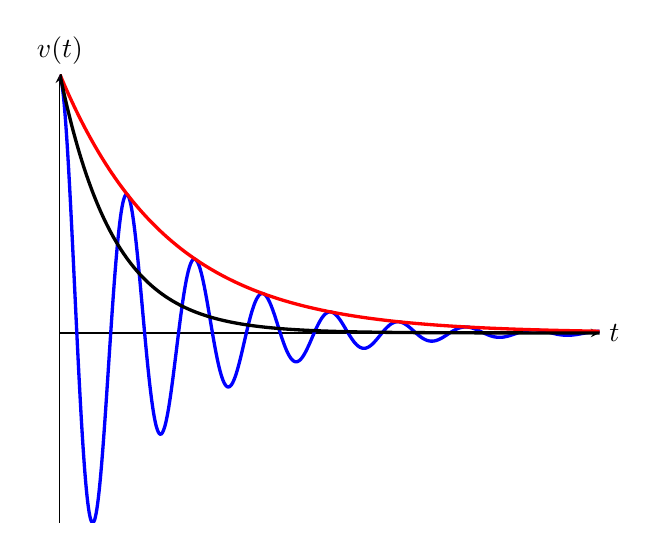
\begin{tikzpicture}
        \begin{axis}[domain=0:5,samples=501,axis lines=center,
        xtick=\empty,ytick=\empty,
        xlabel={$t$},xlabel style={anchor=west},
        ylabel={$v(t)$},ylabel style={anchor=south}]
        \addplot[color=blue,no marks,very thick,smooth] {(exp(-x)*cos(10*deg(x)))};
        \addplot[color=red,no marks, very thick, smooth] {(exp(-x))};
        \addplot[color=black, no marks, very thick, smooth] {(exp(-2 * x))};
        \end{axis}
    \end{tikzpicture}
    }

    \end{enumerate}


%     Solve the differential equation. Considering all of these cases.

% 	\sol{The general solution to the trsolient equation of this form is \[V_{out}(t)=K_1e^{\lambda_1 t}+K_2e^{\lambda_2 t}\]
% 	where
% 	\[\lambda_1=-\alpha +\sqrt{\alpha^2-\omega_0^2}  \]
% 	\[\lambda_2=-\alpha -\sqrt{\alpha^2-\omega_0^2}\]
% 	In this case,
% 	\[\alpha=\frac{1}{2R_sC}\]
% 	\[\omega_0=\frac{1}{\sqrt{LC}}\]
% 	Now to find the constants $K_1$ and $K_2$, we use the initial conditions for $v_{out}(0)$ and $\frac{dv_{out}(0)}{dt}$ and set the general solution to these values:
% 	\begin{align*}
% 		\frac{dv_{out}(0)}{dt}=\frac{V_s}{R_sC}&=K_1\lambda_1+K_2\lambda_2 \\
% 	v_{out}(0)=0&=K_1+K_2 \\
% 	\frac{V_s}{R_sC}&=-K_2\lambda_1+K_2\lambda_2 \\
% 	K_2&=\frac{V_s}{R_sC(\lambda_2-\lambda_1)} \\
% 	K_1&=-\frac{V_s}{R_sC(\lambda_2-\lambda_1)}
% 	\end{align*}
% 	Finally, plugging back into the general solution:
% 	\[V_{out}(t)=-\frac{V_s}{R_sC(\lambda_2-\lambda_1)}e^{\lambda_1 t}+\frac{V_s}{R_sC(\lambda_2-\lambda_1)}e^{\lambda_2 t}\]

% 	For the $\lambda_1=\lambda_2$, which happens in a critically damped system, the general solution is:
% \[V_c=K_1e^{\lambda t}+tK_2e^{\lambda t}\]
% and
% \[\frac{dV_c}{dt}=K_1\lambda e^{\lambda t}+K_2e^{\lambda_t}+t K_2 \lambda e^{\lambda t}\]
% so when plugging our initial conditions into these equations
% \begin{align*}
% V_{out}(0)&=0=K_1 \\
% \frac{dV_c (0)}{dt}&=\frac{V_s}{R_sC}=K_1\lambda+K_2 \\
% K_2&= \frac{V_s}{R_sC} \\
% K_1&=0 \\
% K_2&=\frac{V_s}{R_sC}
% \end{align*}

\newpage
% {\Large \textbf{Mechanical:}}
\qns{Complex Numbers}

A complex number, $z$, is composed of a real part and imaginary part.
If $z = a + bj$, then $re(z) = a$ (the real portion equals a), and $im(z) = b$ (the imaginary portion equals b).
Complex numbers can be expressed in two ways:

\begin{center}
Rectangular Form: $z = a + bj$ \hspace{1em} Polar Form: $z = re^{j\theta}$
\end{center}

In polar form, $r$ represents the magnitude and $\theta$ represents the angle of the complex number with respect to the origin of the complex plane.
Rectangular form makes adding and subtracting complex numbers easier; whereas, polar form makes multiplying and dividing numbers easier.
Some handy equations to switch between forms include:

\begin{center}
\begin{tabular}{ c c c }
 $tan(\theta) = \frac{b}{a}$ & $r = |z| = \sqrt{a^2 + b^2}$ \\ \\
 $sin(\theta) = \frac{b}{|z|}$ & $cos(\theta) = \frac{a}{|z|}$ \\  \\
\end{tabular}
\end{center}

\begin{enumerate}

\qitem Prove algebraically that $\frac{1}{j} = -j$.

\sol{
The key is to multiply the left-hand side of the equation by $\frac{j}{j}$: \\
$$\frac{1}{j} = \frac{1 * j}{j * j} = \frac{j}{j^2}$$
$$= \frac{j}{-1} = -j$$
}

\end{enumerate}

A complex number, $z = a + bj$ has a complex conjugate, $\overline{z} = a - bj$.
Note that the sum of a complex number and its conjugate is always real, but the difference between a complex number and its conjugate is always imaginary.

\begin{enumerate}[resume]

\qitem Use a polar graph to show that the sum of any complex number and its conjugate is always real.

\sol{

}

\qitem Recall that Euler's Formula states that $e^{j\theta} = cos(\theta) + jsin(\theta)$.
Using Euler's identity, show that $cos(\theta) = \frac{1}{2}(e^{j\theta} + e^{-j\theta})$.

\sol{

  $$e^{j\theta} = cos(\theta) + jsin(\theta)$$

  Note that $e^{j\theta}$ has the complex conjugate $e^{-j\theta}$, which means:

  $$e^{-j\theta} = cos(\theta) - jsin(\theta)$$
  $$e^{j\theta} +  e^{-j\theta} = cos(\theta) + jsin(\theta) + cos(\theta) - jsin(theta)$$
  $$e^{j\theta} +  e^{-j\theta} = 2cos(\theta)$$
  $$cos(\theta) = \frac{1}{2}(e^{j\theta} +  e^{-j\theta})$$

}

\end{enumerate}


\end{qunlist}

\end{document}
